% Preamble
\documentclass[12pt,xcolor=dvipsnames]{beamer}

% Packages
\usepackage{amsmath}
\usepackage{graphicx}
\usepackage{listings}
\usepackage{xcolor}
\usepackage{tikz}
\usepackage{pgfplots}
\usetikzlibrary{matrix}
\usetikzlibrary{positioning}

\title{Inside SciPy}
\subtitle{Optimizing Scientific Python}
\date{2025-07-31}
\author{Kai Striega}
\institute{Cartesian Software \& SciPy}

\definecolor{codegreen}{rgb}{0,0.6,0}
\definecolor{codegray}{rgb}{0.5,0.5,0.5}
\definecolor{codepurple}{rgb}{0.58,0,0.82}
\definecolor{backcolour}{rgb}{0.95,0.95,0.92}

\lstdefinestyle{mystyle}{
    backgroundcolor=\color{backcolour},
    commentstyle=\color{codegreen},
    keywordstyle=\color{magenta},
    numberstyle=\tiny\color{codegray},
    stringstyle=\color{codepurple},
    basicstyle=\tiny,
    breakatwhitespace=false,
    breaklines=true,
    captionpos=b,
    keepspaces=true,
    numbers=left,
    numbersep=5pt,
    showspaces=false,
    showstringspaces=false,
    showtabs=false,
    tabsize=4
}

\lstset{style=mystyle}

% Document
\begin{document}

    \maketitle

    \begin{frame}{How to get the slides}
        \begin{itemize}
            \item Available on GitHub
            \item \url{https://github.com/Kai-Striega/speeches/blob/main/inside-scipy-rgi/out/inside_scipy_rgi.pdf}
        \end{itemize}
    \end{frame}

    \begin{frame}{Who am I, and how do I fit in?}
        \begin{itemize}
            \item Hi, I'm Kai!
            \item Maintainer of SciPy since 2018
            \item Senior Software Engineer at Cartesian Software
            \item BSc (Mathematics)
            \item \textbf{Really don't like slow code}
        \end{itemize}
    \end{frame}

    \begin{frame}{What this talk is about}
        \begin{itemize}
            \item Show how we approach performance optimisation
            \item Using SciPy’s RegularGridInterpolator as an example
            \item What we'll cover (quickly)
            \begin{itemize}
                \item Benchmarking
                \item Profiling
                \item Extending Python with native languages
                \item Cython, and Cython optimisations
            \end{itemize}
        \end{itemize}
    \end{frame}

    \begin{frame}{Disclaimers \& Thanks}
        \begin{itemize}
            \item<1-> This is the abridged version
            \item<2-> This is only \textit{partly} my own work
            \item<3-> Co-contributors:
            \begin{itemize}
                \item Evgeni Burovski (@ev-br)
            \end{itemize}
            \item<4-> Reviewers/Mentors:
            \begin{itemize}
                \item Julien Jerphanion (@jjerphan)
                \item Pamphile Roy (@tupui)
            \end{itemize}
        \end{itemize}
    \end{frame}

    \begin{frame}{About SciPy}
        \begin{itemize}
            \item ``Fundamental algorithms for scientific computing in Python''
            \item Free and Open Source
            \item Broadly applicable
            \item Foundational
            \item Easy to use
            \item \textbf{Performant}
        \end{itemize}
    \end{frame}

    \begin{frame}{SciPy: A \textit{performant} Python library?}
        \begin{itemize}
            \item<1-> SciPy wraps highly-optimized implementations written in low-level languages
            \item<1-> Enjoy the flexibility of Python with the speed of compiled code
            \item<1-> Is it performant?
            \item<2-> Yes!
            \item<3-> \ldots \textit{most of the time}
        \end{itemize}
    \end{frame}

    \begin{frame}{Regular Grid Interpolation: One of SciPy's tools}
        \begin{itemize}
            \item SciPy had a function \textit{interp2d}
            \item \textit{interp2d} interpolated points on a regular grid in 2d space
            \item Written in Fortran
            \item It was removed in SciPy 1.14.0 due to being unmaintainable and (very) buggy
        \end{itemize}
        \begin{figure}
            \centering
            \begin{minipage}[b]{0.49\textwidth}
                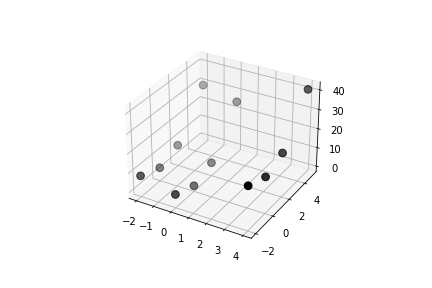
\includegraphics[width=\textwidth]{static/pics/interpolation_points_2d}
                \caption{Some point to interpolate.}
            \end{minipage}
            \hfill
            \begin{minipage}[b]{0.49\textwidth}
                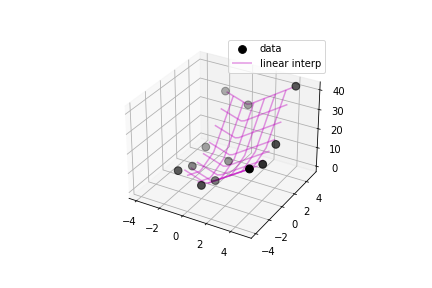
\includegraphics[width=\textwidth]{static/pics/interpolation_2d}
                \caption{The interpolated values.}
            \end{minipage}
        \end{figure}
    \end{frame}

    \begin{frame}{RegularGridInterpolator}
        \begin{itemize}
            \item \textit{interp2d} was replaced by several new classes
            \item One of these is the \textit{RegularGridInterpolator} (RGI) class
            \item Which is user-friendly, written in pure python and less buggy
        \end{itemize}
    \end{frame}

    \begin{frame}{Benchmarking}
        \begin{itemize}
            \item Benchmarking means to evaluate or test a system in order to gain an idea of its performance level.
            \item \textbf{Benchmarking is complicated}
            \item SciPy has its own benchmarking suite based on air speed velocity
            \item All benchmarks were conducted on the same machine with an i9-12900k processor
        \end{itemize}
    \end{frame}

    \begin{frame}{An example us of the \textit{RGI} class}
        \lstinputlisting[language=Python,label={lst:rgi_example}]{static/code_samples/rgi_example.py}
    \end{frame}

    \begin{frame}{Benchmarking Results}
        \begin{center}
        \begin{tabular}{ | c | c | c | }
            \hline
            Scenario & Time (s) & Relative Speedup \\
            \hline
            Raw Python & 36.8 & 1.0 \\
            \hline
        \end{tabular}
        \end{center}
    \end{frame}

    \begin{frame}{Is this \textit{fast}?}
        \begin{itemize}
            \item We had a second function \textit{interp2d}
            \item I originally claimed that this was faster
            \item Let's see how it compares \ldots
        \end{itemize}
    \end{frame}

    \begin{frame}{\textit{interp2d} benchmark result}
        \begin{center}
        \begin{tabular}{ | c | c | c | }
            \hline
            Scenario & Time (s) & Relative Speedup \\
            \hline
            Raw Python & $36.8$ & $1.0$ \\
            interp2d & $11.7$ & $3.17$ \\
            \hline
        \end{tabular}
        \end{center}
    \end{frame}

    \begin{frame}{Is this \textit{fast}?}
        \begin{itemize}
            \item<1-> \textit{interp2d} is $>3$ times faster than \textit{RGI}
            \item<2-> :(
        \end{itemize}
    \end{frame}

    \begin{frame}{Where are we wasting time?}
        \begin{itemize}
            \item A profile is a set of statistics that describes how often and for how long various parts of the program are executed
            \item Useful as we can focus our attention on the slowest parts of the code
            \item We will use Python’s inbuilt \textit{cProfile} module
            \item \ldots but there are many other profilers, I recommend \textit{Scalene}
        \end{itemize}
    \end{frame}

    \begin{frame}{Abridged Profiling Output}
        123 function calls in 63.184 seconds
        \begin{center}
        \begin{tabular}{ | c | c | c | l |}
            \hline
            ncalls & tottime & \% time & function \\
            \hline
            1 & 26.850 & 42 & \_evaluate\_linear \\
            1 & 14.728 & 23 & \_find\_indices \\
            2 & 9.042 & 14 & `searchsorted' of `numpy.ndarray' \\
            & $\vdots$ & & \\
            \hline
        \end{tabular}
        \end{center}
        \begin{itemize}
            \item<2-> Profiling adds \textbf{overhead}; our run has slowed down significantly
            \item<2-> We spend $\approx$ 65\% of time in the functions \_evaluate\_linear and \_find\_indices
            \item<2-> Let's look at those!
        \end{itemize}
    \end{frame}

    \begin{frame}{\textit{\_find\_indicies}}
        \lstinputlisting[language=Python,label={lst:rgi_find_indicies}]{static/code_samples/find_indices.py}
    \end{frame}

    \begin{frame}{\textit{\_evaluate\_linear}}
        \lstinputlisting[language=Python,label={lst:rgi_eval_linear}]{static/code_samples/evaluate_linear.py}
    \end{frame}

    \begin{frame}{Speeding up Python}
        \begin{itemize}
            \item Things to consider:
            \begin{enumerate}
                \item Algorithmic Complexity
                \item More optimal datastructures (np.array vs lists/tuples)
                \item Micro optimisations
            \end{enumerate}
            \item Pure Python $\implies$ computational overhead
            \item Could remove overhead by extending with a low level language
        \end{itemize}
    \end{frame}

    \begin{frame}{Extending Python}
        \begin{itemize}
            \item Manual C/C++ extension module
            \item Fortran + f2py
            \item Numba
            \item Pythran
            \item Cython
        \end{itemize}
    \end{frame}

    \begin{frame}{Cython}
        \begin{itemize}
            \item Compiles a super set of Python to C
            \item Supports optional static type declarations
            \item Allows for very fast program execution
        \end{itemize}
    \end{frame}

    \begin{frame}{Naively Cythonizing}
        \begin{itemize}
            \item Cython can be run on any .py/.pyx file
            \item Generates a .c file with python bindings
            \item What happens if we move \textit{\_evaluate\_linear} and \textit{\_find\_indices} to a .pyx file and compile it?
        \end{itemize}
    \end{frame}

    \begin{frame}{Naive Cython benchmark result}
        \begin{center}
        \begin{tabular}{ | c | c | c | }
            \hline
            Scenario & Time (s) & Relative Speedup \\
            \hline
            Raw Python & 36.8 & 1.0 \\
            interp2d & 11.7 & 3.17 \\
            Naive Cython & 46.4 & 0.79 \\
            \hline
        \end{tabular}
        \end{center}
    \end{frame}

    \begin{frame}{Wait, Cython is slower!?}
        \begin{itemize}
            \item Never seen this before
            \item Don’t really understand why
            \item Hypothesis:
            \begin{itemize}
                \item Some overhead converting Python data to C data
                \item Compiler can’t optimise it well without static typing
                \item Heavy use of Python functions such as ``itertools'', ``zip''
            \end{itemize}
        \end{itemize}
    \end{frame}

    \begin{frame}{Investigating Python Interaction}
        \begin{itemize}
            \item Cython compiles Python to C
            \item This does not mean it avoids the Python interpreter
            \item The interpreter is (usually) slow
            \item ``--annotate'' generates a HTML file that shows us how Cython interacts with the interpreter
            \item Yellow highlighting $\implies$ interaction with the interpreter
        \end{itemize}
    \end{frame}

    \begin{frame}{View the Naive Cython interactions}
        Open the Naive Cython Annotations file
    \end{frame}

    \begin{frame}{Add static typing}
        \begin{itemize}
            \item Cython supports static type annotations
            \item Allows Cython to bypass the dynamic nature of Python
            \item All C types are available for annotation
        \end{itemize}
    \end{frame}

    \begin{frame}{Remove Python specific functions}
        \begin{itemize}
            \item zip
            \item list comprehensions
            \item itertools.product
            \item np.where
            \item np.searchsorted
        \end{itemize}
    \end{frame}

    \begin{frame}{Use memory views}
        \begin{itemize}
            \item Everything in Python is an object
            \item Every Python object contains a pointer to the heap
            \item A list of numbers is a list of pointers to numbers
            \item \ldots which is \textbf{very} slow
            \item Memory views directly store a block of contiguous numbers
        \end{itemize}
    \end{frame}

    \begin{frame}{View the Typed Cython interactions}
        Open the Typed Cython Annotations file
    \end{frame}

    \begin{frame}{Typed Cython benchmark result}
        \begin{center}
        \begin{tabular}{ | c | c | c | }
            \hline
            Scenario & Time (s) & Relative Speedup \\
            \hline
            Raw Python & 36.8 & 1.0 \\
            interp2d & 11.7 & 3.17 \\
            Naive Cython & 46.4 & 0.79 \\
            Typed Cython & 18.8 & 1.95 \\
            \hline
        \end{tabular}
        \end{center}
    \end{frame}

    \begin{frame}{Compiler Directives}
        \begin{itemize}
            \item Compiler directives are instructions that affect the behaviour of the Cython code
            \item Can be used to further speed up the behaviour of the code
            \item Make a trade-off between performance and being Pythonic
        \end{itemize}
        \lstinputlisting[language=Python,label={lst:cython_complier}]{static/code_samples/compiler_directives.py}
    \end{frame}

    \begin{frame}{Final Cython benchmark result}
        \begin{center}
        \begin{tabular}{ | c | c | c | }
            \hline
            Scenario & Time (s) & Relative Speedup \\
            \hline
            Raw Python & 36.8 & 1.0 \\
            interp2d & 11.7 & 3.17 \\
            Naive Cython & 46.4 & 0.79 \\
            Typed Cython & 18.8 & 1.95 \\
            Final Cython & 16.4 & 2.24 \\
            \hline
        \end{tabular}
        \end{center}
    \end{frame}

    \begin{frame}{Consequences}
        \begin{itemize}
            \item Sped up the benchmark by a factor of $\approx$2
            \begin{itemize}
                \item Lower end of gains usually seen with Cython
                \item Hints at large Python interaction
                \item Only Cythonized the parts that are bottlenecks
            \end{itemize}
            \item Added a compilation step to the project
            \begin{itemize}
                \item SciPy already has a compilation step
                \item May matter for your project
            \end{itemize}
            \item Made the code less Pythonic
        \end{itemize}
    \end{frame}

    \begin{frame}
        This work is not finished!
    \end{frame}

    \begin{frame}{Cython benchmark result}
        \begin{center}
        \begin{tabular}{ | c | c | c | }
            \hline
            Scenario & Time (s) & Relative Speedup \\
            \hline
            Raw Python & 36.8 & 1.0 \\
            Naive Cython & 46.4 & 0.79 \\
            Typed Cython & 18.8 & 1.95 \\
            Final Cython & 16.4 & 2.24 \\
            Your Contribution & $?$ & $?$ \\
            \hline
        \end{tabular}
        \end{center}
    \end{frame}

\end{document}
